\documentclass[11pt,a4paper]{article}
\usepackage[utf8]{inputenc}
\usepackage[english]{babel}
\usepackage{a4wide,multirow,url,graphicx,enumitem}

\setlist{noitemsep}

\title{Goal-Models and the i* Modelling Method }

\author{Marie Windhorst}
\date{8 June, 2021}

\parindent0pt
\parskip3pt

\begin{document}

\maketitle

\section{Introduction to Goal Oriented Requirements Engineering}
Requirements engineering is according to the \textit{International
  Organization for Standardization} defined as following:
\begin{quote}\it 
  "interdisciplinary function that mediates between the domains of the
  acquirer and supplier to establish and maintain the requirements to be met
  by the system, software or service of interest.

  NOTE: Requirements engineering is concerned with discovering, eliciting,
  developing, analyzing, determining verification methods, validating,
  communicating, documenting, and managing requirements." \cite[p.6]{.2011}
\end{quote}
Requirements engineering is therefore necessary for a successful development
of a system, program etc., because it defines the requirements that are needed
to meet the intended purpose of the system \cite[p.33]{Singh.2008}. One way to
approach requirements engineering is from a goal oriented perspective. Van
Lamsweerde defines a goal as \textit{"an objective the system under
  consideration should achieve."} \cite[p.250]{vanLamsweerde.2001}. The
system in that case can be either referring to the current system or to the
system-to-be, and both states of the system are of importance in the
requirements engineering process. Van Lamsweerde understands a system as a
composition of the environment. The system is made of active components with
their own behavior \cite{vanLamsweerde.2001}. The active components can be
anything from human, software, institutions or devices and are called
agents. And to make the loop back to the requirements: \textit{"A goal under
  responsibility of a single agent in the software-to-be becomes a
  requirement."} \cite[p.250]{vanLamsweerde.2001}.

It is helpful to use goals as a guideline for requirements engineering process
for the following reasons \cite[p.250]{vanLamsweerde.2001}:
\begin{itemize}
\item to achieve requirements completeness,
\item to avoid irrelevant requirements,
\item to explain requirements to stakeholders,
\item to provide a natural mechanism to structure complex requirements,
\item to find alternative goal refinements,
\item to manage conflicts among multiple viewpoints,
\item to separate stable from unstable information,
\item to use goals as a driving force.
\end{itemize}

One problem with goals is, that often they are not expressed directly, but
more often indirect or informally. A possible approach to identify goals is to
analyze the current system and use it as a source to identify goals. Having a
closer look a the current state of the system might end up in a list of
problems, and simply turning the problems around can provide in a list of
goals to be achieved for the system-to-be \cite[p.250f.]{vanLamsweerde.2001}.

There are several modelling languages that help to analyze, conceptualize and
model the requirements of a system to be developed or transformed. Some of the
well known goal oriented modelling languages are KAOS and i*
\cite{Dardenne.1993, Yu.1995}. The following introduced modelling language i*
(pronounced iStar) was developed by Yu \cite{Yu.1995}. It is based on the
goal modelling approach, but takes it as a starting point for an
agent-oriented modelling language.

\section{An Agent Oriented Modelling Framework -- Introduction to i* Modelling
  Language} 
\subsection{i* -- its idea and intention}
The i* modelling language was developed by Yu \cite{Yu.1995} in his
dissertation published in 1995. The framework is designed for the early-phase
of the requirements engineering process. It builds upon the goal-oriented
framework described above but puts a special emphasis on modelling social
relations, in that sense i* is also an agent-oriented modelling framework. It
is the understanding that a system should aim at improving the relationship
among actors, thus in order for a system to work, the social relations have to
be analyzed beforehand \cite{Yu.2011b}. The early-phase of requirements
engineering is characterized by understanding the motivation to create a
system-to-be, why the current circumstanced do not work and what the different
perspectives are on the current situation. This can be analyzed by looking at
and rearranging the different social relationships involved.

The benefit of applying a social worldview is to see and understand the
different kinds of intentions, dependencies, interests, reasons and many more
of the different actors involved the system(-to-be). Especially vague ideas of
a system-to-be, or simple desires of an actor can be easily added to such a
social worldview. Additionally, applying a social worldview allows to
acknowledge the fact that each actor acts (semi-)autonomously in that sense
that the actor has a behaviour of himself/herself, but is also dependent on
their environment and other actors involved \cite{Yu.2011b}.

The i* modelling framework takes upon the two above mentioned benefits of a
goal and agent oriented perspective. It uses goals to describe the intentions
as attributes of the different actors involved and hence can incorporate the
viewpoints from several perspectives. With dependencies created between
different actors, the autonomy and vulnerability of actors are also
incorporated into the system modelling process. With this combination of goals
and agents it is possible to recognize the possible trade-offs and
opportunities of different/competing goals from several perspectives
\cite{Yu.2011b}.

Currently the version i* 2.0 is used. The new standard was published 2016 and
is under continuous development \cite{Dalpiaz.25.05.2016}. For the i*
modelling language several domain specific extensions are available, thus i*
can be used for many different modelling tasks in many different domains which
shows the intended open nature of i* \cite{Goncalves.2018}.

\subsection{i* Notation -- What can i* model?}
As mentioned before, the focus of i* are the social relations between
different actors involved in a system. A summary of the notation of i* can be
seen in table \ref{Table_1} as well as some example models in figures 1-3 of a
travel reimbursement scenario as described in \cite{Dalpiaz.25.05.2016}.
Generally i* differentiates between the following model views;
\textit{Strategic Rationale, Strategic Dependency, Hybrid SD/SR} (see figures
1--3 for examples).
\begin{itemize}
\item \textit{Strategic Rationale (SR):} This view shows all the links,
  relations, dependencies, resources etc.
\item \textit{Strategic Dependency (SD):} This view only focuses on the actors
  and the associations to others and their dependencies among each other
  including the intentional elements.
\item \textit{Hybrid SD/SR:} The hybrid view is useful, when for example not
  all the information about all actors is available, or the model is defined
  from a specific perspective.
\end{itemize}
From the perspectives of the SR and SD model view, the following section is
going to describe what i* can model and for what it can possibly used for.

\textit{Strategic Dependency Model (SD):} The focus of the SD model is, as its
name already states, the dependencies of the different actors, how they are
related to each other in terms of their dependencies to each other. The
dependency relationship describes a depender, its dependee and the dependum
(compare figure 2 and table 1). The focus on the dependencies allows the
identification of possible vulnerabilities and opportunities resulting from
the different social relations. Taking the example of the travel reimbursement
scenario, the student is dependent on the travel agency to provide the booked
tickets and the trip being booked, which could create a vulnerability for the
student if the travel agency does not do their tasks. But this also offers the
student some leisure, not to worry about the trip being booked.

\textit{Strategic Rationale Model (SR):} The SR model includes all the
dependencies described in the SD model and additionally shows the intentions,
resources, tasks and the like of the different actors (compare figure 2). One
can say that it takes a deeper look into the actors involved and elaborates
their position in the system. Different tasks are decomposed into sub tasks,
linking different actors together, showing how they interrelate to each other
and hierarchically ordered. This could be of special interests to evaluate if
there are any alternatives with respect to the interests and intents of the
actors. As mentioned in the SD model in figure 1, the student is dependent on
the travel agency for them to book the trip. When having a look at the SR
model (see figure 2), it is possible to evaluate why involving a travelling
agency is of comfort for the student: it is is quicker, it is more
comfortable, but also possibly more expensive compared to booking the trip
himself/herself.
\newpage

\subsection{Overview of the i* modelling notation as described in
  \cite{Dalpiaz.25.05.2016}.}\label{Table_1}
  \newcommand{\abox}[1]{\parbox{.5\textwidth}{\vskip6pt #1\vskip6pt}}
  \newcommand{\bbox}[1]{\parbox{3cm}{\raggedright #1}}
\begin{center}
\begin{tabular}{|l|l|l|l|}\hline
  \textbf{Group} & \multicolumn{2}{l|}{\textbf{Variations}} &
    \textbf{Description} \\ \hline

  \multirow{4}{*}{Actors} & \multicolumn{2}{l|}{Actor} & \abox{Autonomous
    entity, that aims at achieving his/her/its goals by exercising their
    know-how, in collaboration with other actors -- used when distinguishing
    the type of actor is not relevant.} \\ \cline{2-4}
    
  & \multicolumn{2}{l|}{Agent} & \abox{Abstract characterization of the
    behavior of a social actor within some specialized context or domain of
    endeavor.}  \\ \cline{2-4}

  & \multicolumn{2}{l|}{Role} & \abox{An actor with concrete, physical
    manifestations, such as human individual, an organization, or a
    department.} \\ \cline{2-4}

  & \multicolumn{2}{l|}{Actor Boundary} & \abox{Visualization for the actors
    intentionality, grouping together their intentional elements together with
    their relationships} \\ \hline

  \multirow{2}{*}{\bbox{Actor Association Links}} & \multicolumn{2}{l|}{Is-a}
  & \abox{Represents the concept of generalization/specialization.}
  \\ \cline{2-4}

  & \multicolumn{2}{l|}{Participates-in} & \abox{Represents any kind of
    association, other than generalization/specialization between actors.  No
    restrictions on type of actor linked.  Source = agent, then the target is
    a role - represents the play relationship.  Source and Target = same type
    - represents part-of relationship. Every actor can participate in multiple
    other actors.}  \\ \hline
  
  \multirow{4}{*}{\bbox{Intentional Elements}} & \multicolumn{2}{l|}{Goal} &
  \abox{State of affairs that the actor wants to achieve and that has
    clear-cut criteria of achievement.} \\ \cline{2-4}
  
  & \multicolumn{2}{l|}{Quality} & \abox{An attribute for which an actor
    desires some level of achievement. The level of achievement may be defined
    precisely or kept vague.} \\ \cline{2-4}
  
  & \multicolumn{2}{l|}{Task} & \abox{Represents actions that an actor wants
    to be executed, usually with the purpose of achieving some goal.}
  \\ \cline{2-4}
  
  & \multicolumn{2}{l|}{Resource} & \abox{A physical informational entity that
    the actor requires in order to perform a task.} \\ \hline
\end{tabular}
\end{center}

\begin{center}
\begin{tabular}{|l|l|l|l|}\hline
  \multirow{5}{*}{\bbox{Social Dependencies}} & \multicolumn{2}{l|}{Depender}
  & \abox{The actor that depends for something (the dependum) to be provided.}
  \\ \cline{2-4}
  
  & \multicolumn{2}{l|}{Depender Element} & \abox{The intentional element
    within the depender's actor boundary where the dependency starts from,
    which explains why the dependency exists.}  \\ \cline{2-4}
  
  & \multicolumn{2}{l|}{Dependum} & \abox{An intentional element that is the
    object of the dependendy. The type of the dependum specializes the
    semantics ot the relationship (e.g. dependum = resource - the dependee is
    expected to make the resource available to the depender; dependum = goal -
    the dependee is expected to achieve the goal, and is free to choose how).}
  \\ \cline{2-4}
  
  & \multicolumn{2}{l|}{Dependee} & {The actor that should provide the
    dependum.}  \\ \cline{2-4}
  
  & \multicolumn{2}{l|}{Dependee Element} & \abox{The intentional element
    that explains how the dependee intends to provide the dependum.} \\ \hline
\end{tabular}
\end{center}

\begin{center}
\begin{tabular}{|l|l|l|l|}\hline
  \multirow{10}{*}{\bbox{Intentional Element Links}} &
  \multicolumn{2}{l|}{Refinement} & \abox{Links goals and tasks
    hierarchically.  Is an $n$-ary relationship relating to one parent to one
    or more children. Parent can only be AND or OR refined, not both at the
    same time.} \\ \cline{3-4}
  
  & \multirow{2}{*}{} & {AND} & \abox{The fulfillment of all the $n$ children
    makes the \\ parent fulfilled.} \\ \cline{3-4}
  
  && {OR} & \abox{Inclusive: the fulfillment of at least one child makes the
    parent fulfilled. Allows for one single child.} \\ \cline{2-4}
  
  & \multicolumn{2}{l|}{Needed By} & \abox{Links a task with a resource and it
    indicates that \\ the actor needs the resource in order to execute the
    task.} \\ \cline{2-4}
  
  & \multicolumn{2}{l|}{Contribution} & \abox{Represents the effects of
    intentional elements on qualities, and are essential to assist analysts in
    the decision-making process among alternative goals or tasks. Defined as
    relationships from a source intentional element to a target quality.}
  \\ \cline{3-4}
  
  & \multirow{4}{*}{} & {Make} & \abox{The source provides sufficient positive
    evidence for the satisfaction of the target.} \\ \cline{3-4}
  
  &&{Help} & \abox{The source provides weak positive evidence for the
    satisfaction of the target.}  \\ \cline{3-4}
  
  &&{Hurt} & \abox{multicolumnThe source provides weak evidence against the
    satisfaction/denial of the target.} \\ \cline{3-4}
  
  &&{Break} & \abox{The source provides sufficient evidence against the
    satisfaction/denial of the target.} \\ \cline{2-4}
  
  & \multicolumn{2}{l|}{Qualification} & \abox{Relates a quality to its
    subject (task, goal, resource). Expresses a desired quality over the
    execution of a task, the achievement of the goal or the provision of the
    resource.}  \\\hline
\end{tabular}
\end{center}

\begin{figure}[ht]
    \centering
    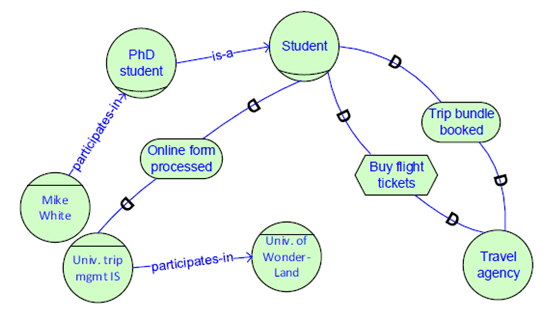
\includegraphics[width=0.8\textwidth]{sdModel.png}
    \caption{Strategic Dependency Model View of a travel reimbursement
      scenario \cite{Dalpiaz.25.05.2016}.}
    \label{fig:my_label2}
\end{figure}

\begin{figure}[ht]
    \centering
    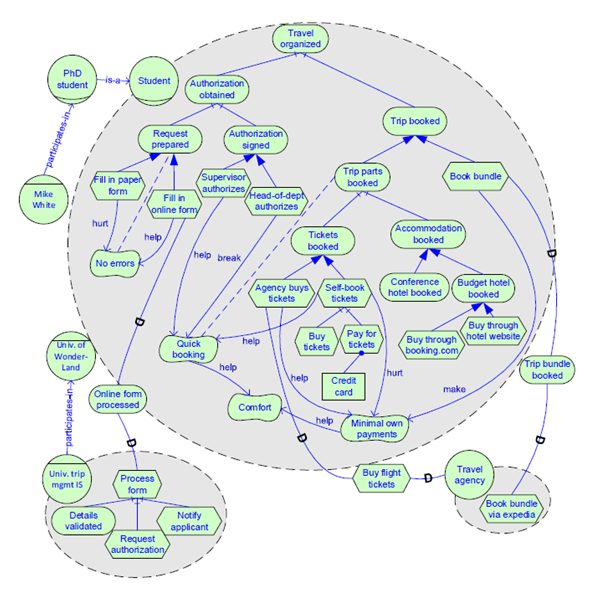
\includegraphics[width=0.9\textwidth]{fullmodelistar.png}
    \caption{Strategic Relationale Model view of a travel reimbursement
      scenario \cite{Dalpiaz.25.05.2016}.}
    \label{fig:my_label1}
\end{figure}

\begin{figure}[ht]
    \centering
    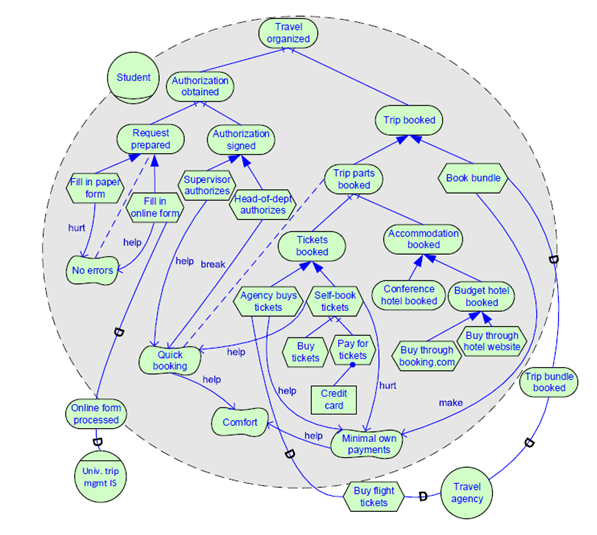
\includegraphics[width=0.8\textwidth]{hybridModel.png}
    \caption{Hybrid SR/SD Model View a travel reimbursement scenario
      \cite{Dalpiaz.25.05.2016}.}
    \label{fig:my_label3}
\end{figure}

\subsection{Short evaluation of the i*}
Although i* is widely used in the research field of requirements engineering,
some recent studies show that it still has some open issues to be
resolved. Yasin and Liu have evaluated a number of studies on i*
\cite{Yasin.2017}. Their findings show, that currently open problems dealt
with in their evaluated studies of i* are concerning the scalability, clarity
and the combined use of i*. Abrah{\~a}o et al. have compared i* 2.0 to
value@GRL concerning several aspects like usability and the achieved model
quality (value@GRL is a simplified i* version) \cite{Abrahao.2019}.  Their
results show that the models created with value@GRL are significantly of
better quality; the participants in the studie found value@GRL more useful;
the ease of use and of value@GRL and i* and productivity of the participant
(productivity = quality and time) are comparable; and last modelling time was
lower for i*.

These findings show that i* seems not to be the answer to all requirements
engineering questions and concerns. But never the less, i* is still very
popular with the research field of goal oriented requirements engineering
\cite[p. 143]{Horkoff.1213.09.2016}.


\section{Conclusion on goal oriented requirements engineering}
Mavin et al. have done a study on the application of goal oriented
requirements engineering in practice \cite{Mavin.2017}. They show that though
it is quite popular in the academic research field, it finds little
application in industry. Most of the publications about goal oriented
requirements engineering are coming from the academic field and only in some
cases show a connection to the industry and actual application of it. A
questionnaire done with practitioners shows that they do work with goal
oriented requirements engineering, but mostly in a more general sense of
goals. This underlines that there is a gap between the academic field on
requirements engineering and its actual application in the field of
industry. Therefore in theory goal oriented requirements engineering seems to
work, but still needs to find a way into the real world.

\bibliographystyle{plain}
\begin{thebibliography}{xxx}
\bibitem{Abrahao.2019} Silvia Abrah{\~a}o, Emilio Insfran, Fernando
  Gonz{\'a}lez-Ladr{\'o}n-de Guevara, Marta Fern{\'a}ndez-Diego, Carlos
  Cano-Genoves, Raphael {Pereira de Oliveira}.  \newblock Assessing the
  effectiveness of goal-oriented modeling languages: A family of experiments.
  \newblock {\em Information and Software Technology}, 116:1--44, 2019.

\bibitem{Dalpiaz.25.05.2016} Fabiano Dalpiaz, Xavier Franch, Jennifer Horkoff.
  \newblock istar 2.0 language guide.  \newblock
  \url{http://arxiv.org/pdf/1605.07767v3}.

\bibitem{Dardenne.1993} Anne Dardenne, Axel {van Lamsweerde}, Stephen Fickas.
  \newblock Goal-directed requirements acquisition.  \newblock {\em Science of
    Computer Programming}, 20(1-2):3--50, 1993.

\bibitem{.2011} International~Organization for Standardization.  \newblock
  {\em Systems and software engineering: Life cycle processes : requirements
    engineering = Ing{\'e}nierie des syst{\`e}mes et du logiciel : processus
    de cycle de vie : ing{\'e}nierie des exigences}.  \newblock ISO and IEC
  and {Institute of Electrical and Electronics Engineers}, Geneva and New
  York, first edition, 2011-12-01 edition, 2011.

\bibitem{Goncalves.2018} Enyo Gon{\c{c}}alves, Jaelson Castro, Jo{\~a}o
  Ara{\'u}jo, Tiago Heineck.  \newblock A systematic literature review of
  istar extensions.  \newblock {\em Journal of Systems and Software},
  137:1--33, 2018.

\bibitem{Horkoff.1213.09.2016} Jennifer Horkoff, Neil Maiden.  \newblock
  Creative leaf: A creative istar modeling tool.  \newblock In Lidia
  L{\'o}pez, Yijun Yu (eds.), {\em Proceedings of the Ninth International i*
    Workshop co-located with 24th International Conference on Requirements
    Engineering (RE 2016)}, CEUR Workshop Proceedings, pp. 25--30.
  CEUR-WS.org, 12-13.09.2016.

\bibitem{Mavin.2017} Alistair Mavin, Philip Wilkinson, Sabine Teufl, Henning
  Femmer, Jonas Eckhardt, Jakob Mund.  \newblock Does goal-oriented
  requirements engineering achieve its goal?  \newblock In Fabiano Dalpiaz,
  Henning Femmer, Andreas Vogelsang (eds.), {\em 2017 IEEE 25th International
    Requirements Engineering Conference Workshops}, pp. 174--183, Piscataway,
  NJ, 2017. IEEE.

\bibitem{Singh.2008} Yogesh Singh, Anjana Gosain, Manoj Kumar.  \newblock
  Evaluation of agent oriented requirements engineering frameworks.  \newblock
  In Stephanie Kawada (ed.), {\em 2008 International Conference on Computer
    Science and Software Engineering}, pp. 33--38, Piscataway, NJ, 2008. IEEE.

\bibitem{vanLamsweerde.2001} A.~{van Lamsweerde}.  \newblock Goal-oriented
  requirements engineering: a guided tour.  \newblock In {\em Proceedings
    Fifth IEEE International Symposium on Requirements Engineering}, pages
  249--262, 2001.

\bibitem{Yasin.2017} Affan Yasin, Lin Liu.  \newblock Recent studies on i*: A
  survey.  \newblock In Sepideh Ghanavati, Lin Liu, Lidia L{\'o}pez (eds.),
  {\em Proceedings of the 10th International i* Workshop co-located with the
    29th International Conference on Advanced Information Systems Engineering
    (CAiSE 2017), Essen, Germany, June 12-13, 2017}, CEUR Workshop
  Proceedings, pp. 1--6. CEUR-WS.org, 2017.

\bibitem{Yu.1995} Eric S.~K. Yu.  \newblock {\em Modeling Strategic
  Relationships for Process Reengineering}.  \newblock PhD thesis, {University
  of Toronto}, Toronto, Canada, 1995.

\bibitem{Yu.2011b} Eric S.~K. Yu, Paolo Giorgini, Neil Maiden, John
  Mylopoulos.  \newblock Social modeling for requirements engineering: An
  introduction.  \newblock In Eric S.~K. Yu (ed.), {\em Social modeling for
    requirements engineering}, Cooperative information systems, pp.  3--10.
  {MIT Press}, Cambridge, Mass., 2011.
\end{thebibliography}
\end{document}
